\chapter{Facial expression recognition in Video}
\minitoc


\section{Introduction}
In this chapter, we applied the proposed method in chapter \ref{Ch_4} to the DynEmo video database. We investigated methods of smoothing the classifier predictions to exploit temporal continuity of emotions and therefore the classification error. Several smoothing techniques were investigated and optimised.

The field of video automatic facial expression analysis has overgrown in recent years. Nevertheless, most researchers still depend on databases that contain acted emotions from models or actors \citep{dhall2013emotion,dhall2014emotion,dhall2015video,dhall2016emotiw}. It is clear by comparing the way facial expressions are expressed in real life are different than those were acted in most databases. 
A recent interesting database showing real facial expression is the DynEmo database \citep{tcherkassof2013dynemo} which was created by a multidisciplinary team of psychological researchers, computer scientists, statisticians, experimentation and instrumentation specialists, and a legal professional. The DynEmo database contains dynamic and natural emotional facial expressions, and filmed in natural but standardised conditions \citep{tcherkassof2013dynemo}. 

% These are divided into two groups of 233 and 125 recordings of emotional facial expressions of ordinary Caucasian people (ages 25 to 65, 182 females and 176 males) filmed in natural but standardised conditions. 



In this chapter, section \ref {database_preparation}  will show how the DynEmo database has been prepared to be usable in our work. In section  \ref{sec:Vid_Experiments} we show the result of applying the proposed method in the previous chapter to the new video database. Section \ref{smooting_PP} which shows how smoothing the classifier scores improves the accuracy.  Finally, conclusions are drawn in section \ref{sec:ch5_Summary}. 

%%%%%%%%%%%%%%%%%%%%%%%%%%%%%%%%%%%%%%%%%%%%%%%%%%
%%%%%%%%%%%%%%%%%%%%%%%%%%%%%%%%%%%%%%%%%%%%%%%%%%
%%%%%%%%%%%%%%%%%%%%%%%%%%%%%%%%%%%%%%%%%%%%%%%%%%
\section{DynEmo database preparation}
\label{database_preparation}

DynEmo database has been labelled over time not frame by frame. In our experiments, we need labelled frames to be used for training and testing.
The researchers in the DynEmo database worked on the following facial expression expressions in the DynEmo database are Curiosity, happy, Surprise, Boredom, Disgust, Fright, Shame, Annoyance, Disappointment, Humiliation. To collect the data, the researchers have recorded films using hidden cameras while people (called encoders) were sitting on a chair at a small table facing the wall where a PC was projected on the wall using a video projector as illustrated in figure \ref{fig:recording_room}. During the video playback, experimenters were sitting in an adjacent room watching the encoders reaction. There recorded videos properties are width: 768, height: 576, frame rate: 25 frames per second, bits per pixel: 24 and video format:'RGB24'. 

%%%%%%%%%%%%%%%%%%%%%%%%%%%%%%%%%%%%%%%%%%%%%%%%%%%%%%%%%%%%%%%%%
\begin{figure}[tb]
	\centering
	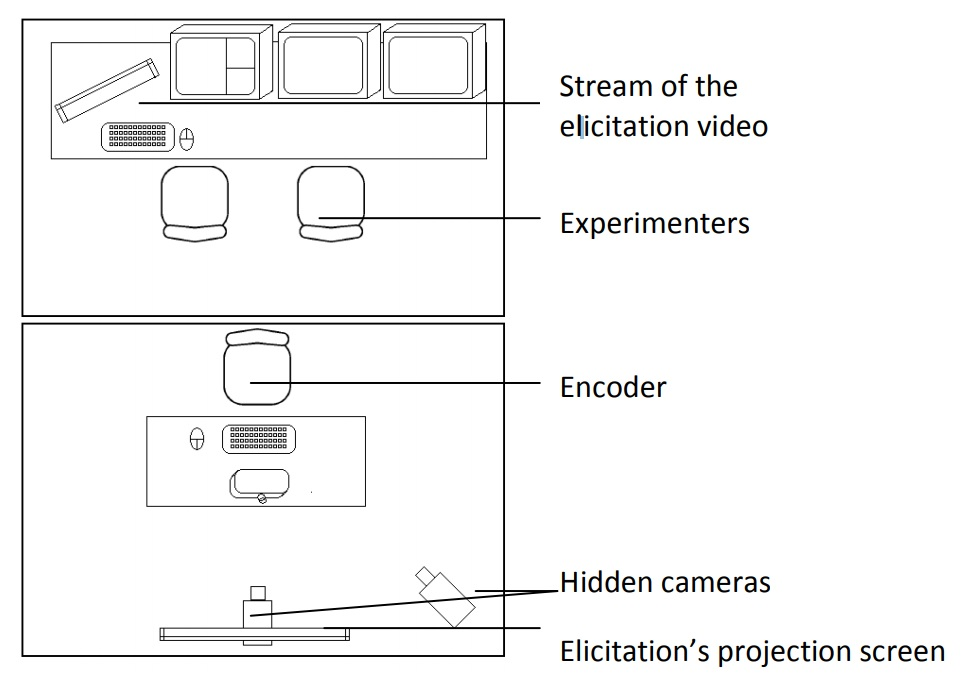
\includegraphics[width=120.5mm]{Chapter5/Figs/recording_room.jpg}
	\textbf{\caption{\label{fig:Emotionalexpressive_time-line}Design of the technical and recording rooms 
			\citep{tcherkassof2013dynemo}.}\label{fig:recording_room}}
\end{figure}
%%%%%%%%%%%%%%%%%%%%%%%%%%%%%%%%%%%%%%%%%%%%%%%%%%%%%%%%%%%%%%%%%




Table \ref{Original_Data} shows a sample of original data layout in the DynEmo database. The most important columns for us in the data are C\_Video which means the video name, E\_Detectee is the labelled emotion, TC\_Debut and TC\_Fin the start and end time by milliseconds. Figure \ref{fig:Emotionalexpressive_time-line} shows an example for a labelled video on the time-line.  On the DynEmo website all videos clips, but only 52 clips are available with labelling data. So in our work, we used the 44 clips as we mentioned.  The first objective is to make the labelling based on frames rather than time. Moreover,  to ensure that there is a consensus on the judgements on each frame.  Work has started by preparing the database to be usable in training and testing. 

%%%%%%%%%%%%%%%%%%%%%%%%%%%%%%%%%%%%%%%%%%%%%%%%%%%%%%%%%%%%%%%%%
\begin{figure}[tb]
	\centering
	\includegraphics[width=120.5mm]{Chapter5/Figs/time-line.png}
	\textbf{\caption{\label{fig:Emotionalexpressive_time-line}Emotional expressive time-line. Frames are taken from the video of an encoder who reported disgust and its corresponding underneath time-line 
			\citep{tcherkassof2013dynemo}.}\label{fig:Emotionalexpressive_time-line}}
\end{figure}
%%%%%%%%%%%%%%%%%%%%%%%%%%%%%%%%%%%%%%%%%%%%%%%%%%%%%%%%%%%%%%%%%


%disgust and its corresponding underneath time-line 
%\citep{tcherkassof2013dynemo}.}
% \centering
%\includegraphics[width=0.7\textwidth]{}
%\caption{\label{fig:Emotionalexpressive_time-line}Emotional expressive time-line. Frames are taken from the video of an encoder who reported
%disgust and its corresponding underneath time-line 
%\citep{tcherkassof2013dynemo}.}
%\end{figure}
% 


\begin{table}[tb]
	\centering
	\textbf{
		\caption{DynEmo database data type.}\label{Original_Data}} \fontsize{7pt}{7pt}
	\selectfont
	\resizebox{\textwidth}{!}{
		\begin{tabular}{@{}|l|l|l|l|l|l|l|l|@{}}
			\toprule
			\textbf{C\_INDUC} & \textbf{SEX\_Sujet} & \textbf{SEXE\_Juge} & \textbf{C\_Juge} & \textbf{C\_Video} & \textbf{E\_Detectee} & \textbf{TC\_Debut} & \textbf{TC\_Fin} \\ \midrule
			EM                & F                   & N                   & 237              & DVD3\_5.mpg       & Stupefaction         & 7181               & 10183            \\ \midrule
			EM                & F                   & N                   & 237              & DVD3\_5.mpg       & Stupefaction         & 23438              & 29080            \\ \midrule
			EM                & F                   & N                   & 237              & DVD3\_5.mpg       & Stupefaction         & 39798              & 50305            \\ \midrule
			EM                & F                   & N                   & 237              & DVD3\_5.mpg       & Ennui                & 60543              & 64007            \\ \midrule
			EM                & F                   & N                   & 237              & DVD3\_5.mpg       & Stupefaction         & 96104              & 99176            \\ \midrule
			EM                & F                   & N                   & 237              & DVD3\_5.mpg       & Stupefaction         & 119316             & 123280           \\ \midrule
			EM                & F                   & N                   & 133              & DVD3\_5.mpg       & Stupefaction         & 4929               & 19463            \\ \midrule
			EM                & F                   & N                   & 133              & DVD3\_5.mpg       & Ennui                & 23241              & 30631            \\ \midrule
			EM                & F                   & N                   & 133              & DVD3\_5.mpg       & Ennui                & 66760              & 70727            \\ \midrule
			EM                & F                   & N                   & 133              & DVD3\_5.mpg       & Curiosite            & 87825              & 91947            \\ \midrule
			EM                & F                   & N                   & 133              & DVD3\_5.mpg       & Ennui                & 94415              & 95537            \\ \midrule
			EM                & F                   & N                   & 133              & DVD3\_5.mpg       & Curiosite            & 110200             & 117211           \\ \midrule
			EM                & F                   & N                   & 133              & DVD3\_5.mpg       & Curiosite            & 121754             & 123280           \\ \midrule
			EM                & F                   & N                   & 229              & DVD3\_5.mpg       & Stupefaction         & 6866               & 12845            \\ \midrule
			EM                & F                   & N                   & 229              & DVD3\_5.mpg       & Stupefaction         & 24385              & 30130            \\ \bottomrule
	\end{tabular}}
\end{table}



Smiler to the work in chapter 3, we need to ensure that there is consensus on the facial expression on each frame. To achieve this, each frame must be assigned on emotion at least four different judges. To qualify the quality of the consensus we calculate the entropy value for the votes. The entropy must be less than $1$ to accept the consensus vote. The entropy for $n$ probabilities $(p_1,p_2, ... ,p_n)$ is calculated by using this equation:



%%%%%%%%%%%%%%%%%%%%%%%%%%%%%%%%%%%%%%%%%%%%%%%%%%%%%%%%%%%%%%%%%
\begin{equation}
H =- \sum_{i=1}^{n}  p_i  \log_2 (p_i)
\end{equation}
%%%%%%%%%%%%%%%%%%%%%%%%%%%%%%%%%%%%%%%%%%%%%%%%%%%%%%%%%%%%%%%%%
where \textit{$p$}; is the fraction of judges voting for class $i$.


We adapted the labelling way to be based in every single frame rather than the original method which was based on time sectors. 
Form the 52 videos available we got 44 videos that they include 14543 frames have been voted with consensus $(entropy<1)$. We removed some short parts of the 44 videos which have no consensus $(entropy>1)$. Some videos have multiple than one expression during the video, so we cut some short part from those videos which have not got consensus. Only five facial emotion remaining after calculating the entropy: Fear, anger, disgust, happy and surprise.      

%So for each frame, we counted how many judgements have elected the expression for each frame. Only frames with less than one entropy are shown in the table, any frame with more than one entropy value means there is no consensus on that frame, So it was excluded.


Natural facial expressions are vary even for the same person, for example, smile expression has many levels. The same person may express a small smile or wide smile. Some people try to hide their expressions sometimes, so this causes facial expression variation. This variation is a big challenge for natural facial expressions recognition. Figures \ref{fig:SamePersonSmile1}, \ref {fig:SamePersonSmile2} and \ref {fig:SamePersonSmile3} show happy expression variation for the same person from the DynEmo database. In most unnatural expression databases,  the actors express a very similar way to show facial expression. %Figures \ref{fig:DeffePersomSmile1}, \ref {fig:DeffePersomSmile2} and \ref {fig:DeffePersomSmile3} show happy expression variation for for three different persons from DynEmo database. 


 DynEmo preparation process has produced 44 videos have been labelled depending on the frame rather than time. Table \ref{table:NewVidDatastatistics} illustrates the new dataset, which contains 14543 frames distributed on five facial expressions as 8902 frames balled as happy, 313 as fear, 2192 as angry, 2665 as surprise and 471 as disgust. Figure \ref{fig:NewDynEmoExample} shows examples of new labelled frames. We used this obtained data in the experiments described in section \ref{sec:Vid_Experiments}.

\begin{table}[tb]
	\centering
	\textbf{
		\caption{General statistics about the new database}\label{table:NewVidDatastatistics}}
	\resizebox{\textwidth}{!}{
		\begin{tabular}{|c|c|c|c|c|l|}
			\hline
			\textbf{Number of videos} & \textbf{Happy frames} & \textbf{Fear frames} & \textbf{Anger frames} & \textbf{Surprise frames} & \textbf{Disgust frames}  \\ \hline
			44                        & 8902                  & 313                 & 2192                  & 2665                     & \multicolumn{1}{c|}{471} \\ \hline
	\end{tabular}}
\end{table}



\begin{figure}
	\resizebox{\textwidth}{!}{
		\begin{tabular}{ccccc}
			Happy &  Fear &  Anger &  Surprise &  Disgust \\[12pt]
			
			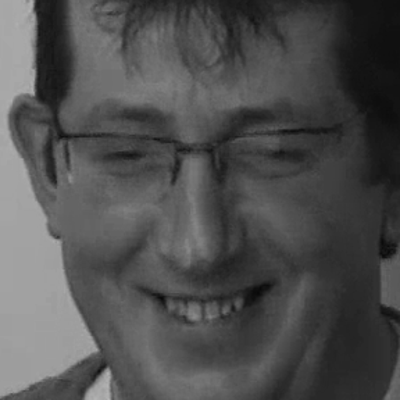
\includegraphics[width=30mm]{Chapter5/Figs/Hap.png} &   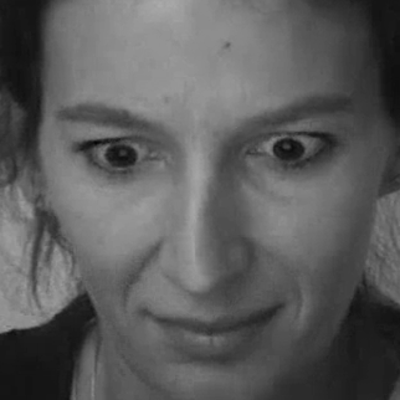
\includegraphics[width=30mm]{Chapter5/Figs/Fear.png}  &   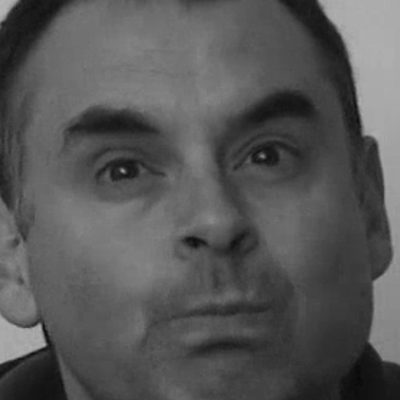
\includegraphics[width=30mm]{Chapter5/Figs/Ang.png} &   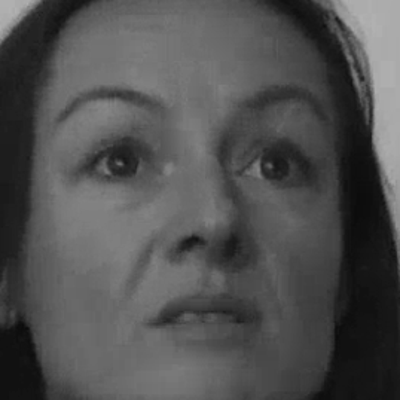
\includegraphics[width=30mm]{Chapter5/Figs/Sur.png}&   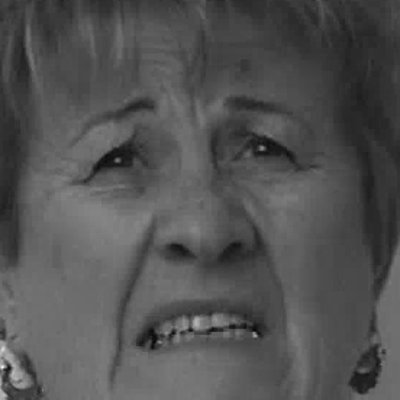
\includegraphics[width=30mm]{Chapter5/Figs/Dis.png}   \\
			
	\end{tabular}}
	\caption{Examples of the five facial expression in the database}
	\label{fig:NewDynEmoExample}
	
\end{figure}

\begin{figure*}[tb]
	\centering
	\begin{subfigure}[t]{0.3\textwidth}
		\centering
		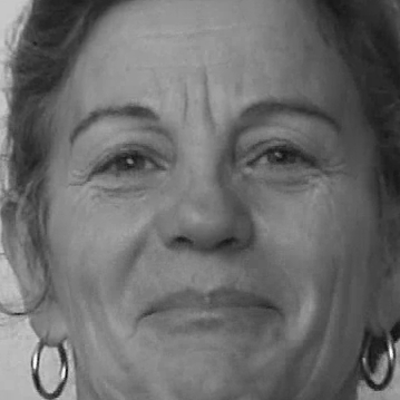
\includegraphics[height=1.2in]{Chapter5/Figs/SamePersonSmile1.png}
		\caption{Low smile.}
		\label{fig:SamePersonSmile1}
	\end{subfigure}%
	~ 
	\begin{subfigure}[t]{0.3\textwidth}
		\centering
		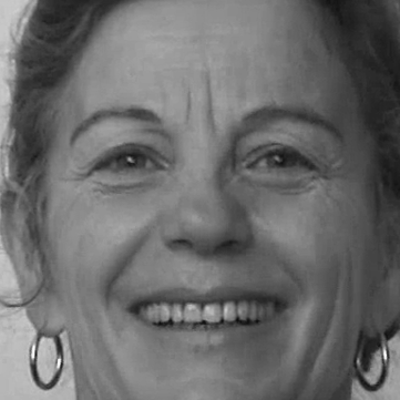
\includegraphics[height=1.2in]{Chapter5/Figs/SamePersonSmile2.png}
		\caption{Average smile.}
		\label{fig:SamePersonSmile2}
	\end{subfigure}
	\begin{subfigure}[t]{0.3\textwidth}
		\centering
		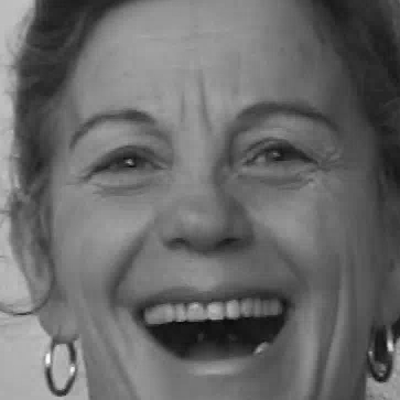
\includegraphics[height=1.2in]{Chapter5/Figs/SamePersonSmile3.png}
		\caption{Wide smile (laugh).}
		\label{fig:SamePersonSmile3}
	\end{subfigure}
	
	\caption{Happy expression variation for the same person.}
\end{figure*}


%\begin{figure*}[t]
%    \centering
%    \begin{subfigure}[t]{0.3\textwidth}
%        \centering
%        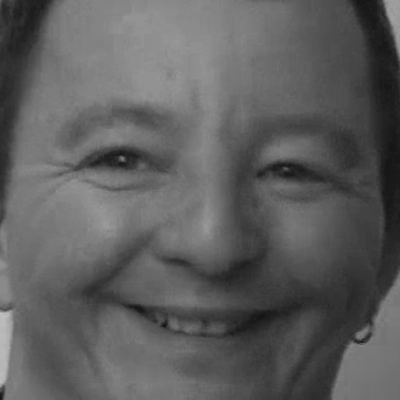
\includegraphics[height=1.2in]{Chapter5/Figs/DeffePersomSmile1.png}
%        \caption{First person smile.}
%         \label{fig:DeffePersomSmile1}
%    \end{subfigure}%
%    ~ 
%    \begin{subfigure}[t]{0.3\textwidth}
%        \centering
%        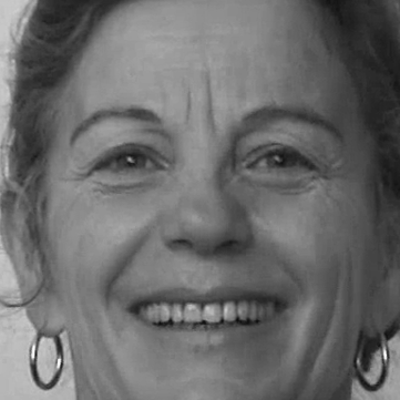
\includegraphics[height=1.2in]{Chapter5/Figs/SamePersonSmile2.png}
%        \caption{Second person smile.}
%        \label{fig:DeffePersomSmile2}
%    \end{subfigure}
%    \begin{subfigure}[t]{0.3\textwidth}
%        \centering
%        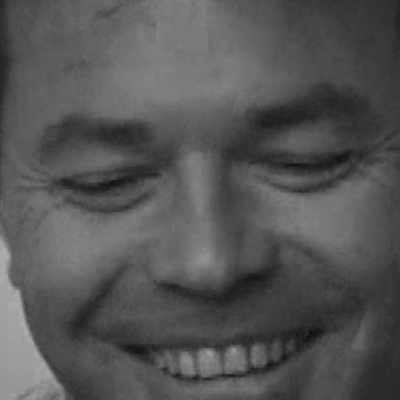
\includegraphics[height=1.2in]{Chapter5/Figs/DeffePersomSmile3.png}
%        \caption{Third person smile.}
%        \label{fig:DeffePersomSmile3}
%    \end{subfigure}
%    
%    \caption{Happy expression variation for three different persons.}
%\end{figure*}




%
%\begin{table}[H]
%\centering
%\textbf{
%\caption{Sample of the new data type labelled by frame.}\label{MyTable2}}
%\selectfont
%\resizebox{\textwidth}{!}{
%\begin{tabular}{@{}|l|l|l|l|l|l|l|l|l|l|l|l|l|l|@{}}
%\toprule
%Frame & Curiosity & Disappointment & Disgust & Be moved & Boredom & Fright & Shame & Anger & Satisfaction & Humiliation & Happy & Stupefaction & RAS \\ \midrule
%3830  & 1         & 0              & 0       & 0        & 0       & 0      & 0     & 0         & 0            & 0           & 0         & 4            & 0         \\ \midrule
%3831  & 1         & 0              & 0       & 0        & 0       & 0      & 0     & 0         & 0            & 0           & 0         & 4            & 0         \\ \midrule
%3832  & 1         & 0              & 0       & 0        & 0       & 0      & 0     & 0         & 0            & 0           & 0         & 4            & 0         \\ \midrule
%3833  & 1         & 0              & 0       & 0        & 0       & 0      & 0     & 0         & 0            & 0           & 0         & 4            & 0         \\ \midrule
%3834  & 1         & 0              & 0       & 0        & 0       & 0      & 0     & 0         & 0            & 0           & 0         & 4            & 0         \\ \midrule
%3835  & 1         & 0              & 0       & 0        & 0       & 0      & 0     & 0         & 0            & 0           & 0         & 4            & 0         \\ \midrule
%3985  & 0         & 0              & 1       & 0        & 0       & 1      & 0     & 0         & 0            & 0           & 17        & 2            & 0         \\ \midrule
%3986  & 0         & 0              & 1       & 0        & 0       & 1      & 0     & 0         & 0            & 0           & 17        & 2            & 0         \\ \midrule
%3987  & 0         & 0              & 1       & 0        & 0       & 1      & 0     & 0         & 0            & 0           & 17        & 2            & 0         \\ \midrule
%3988  & 0         & 0              & 1       & 0        & 0       & 1      & 0     & 0         & 0            & 0           & 17        & 2            & 0         \\ \midrule
%3989  & 0         & 0              & 1       & 0        & 0       & 1      & 0     & 0         & 0            & 0           & 17        & 2            & 0         \\ \midrule
%3990  & 0         & 0              & 1       & 0        & 0       & 1      & 0     & 0         & 0            & 0           & 17        & 2            & 0         \\ \midrule
%3991  & 0         & 0              & 1       & 0        & 0       & 1      & 0     & 0         & 0            & 0           & 17        & 2            & 0         \\ \midrule
%3992  & 0         & 0              & 1       & 0        & 0       & 1      & 0     & 0         & 0            & 0           & 17        & 2            & 0         \\ \midrule
%3993  & 0         & 0              & 1       & 0        & 0       & 1      & 0     & 0         & 0            & 0           & 17        & 2            & 0         \\ \bottomrule
%\end{tabular}}
%\end{table}





%\begin{figure}[ht]
%\centering
%\includegraphics[width=0.7\textwidth]{time-line.png}
%\caption{\label{fig:Emotionalexpressive_time-line}Emotional expressive time-line. Frames are taken from the video of an encoder who reported
%disgust and its corresponding underneath time-line 
%\citep{tcherkassof2013dynemo}.}
%\end{figure}







%%%%%%%%%%%%%%%%%%%%%%%%%%%%%%%%%%%%%%%%%%%%%%%%%%
%%%%%%%%%%%%%%%%%%%%%%%%%%%%%%%%%%%%%%%%%%%%%%%%%%
%%%%%%%%%%%%%%%%%%%%%%%%%%%%%%%%%%%%%%%%%%%%%%%%%%

%    
%    
%\clearpage
%\newpage 


\section{Video Classification Experiments}
\label{sec:Vid_Experiments}
In our experiments, we used five facial expressions: happy, fear, angry, surprise and disgust. We trained our proposed system on videos and photos containing the five facial expressions. Because the videos are sequences of frames, we do not need to train the system using all frames,  so we chose only one frame of each 25 from happy, anger and surprise and all fear and disgust frames, then we add to each class of the training data 70 images from KDEF and 70 images from eLFW. It is important to know that in the testing we have never used any video for testing and training at the same time. This training and testing were repeated five times (5-fold cross-validation), each time leaving different complete videos out for testing, and training with the remaining videos mixed with KDEF and eLFW images. 

A trained Random forest model has been used to predict testing videos, and this returns scores for all training classes. Scores (posterior probability generated by each tree is a matrix with one row per observation and one column per class.
Figure \ref{fig:Classifier_prediction} shows a prediction behaviour of random frosts classier with two happy-labelled videos (DVD31\_1 and DVD14\_). Random Frosts returned voting values (scores) for each frame referring to the training classes.
Table \ref{tab:ConfusionmatrixbeforeSmmoth} right shows two confusion matrices, the left for one RF classifier and the right shows a confusion matrix for 10 pairwise classifiers. In the left table, the happy expression was the best rate with $85\%$ accuracy, and fear like static images was the lowest accuracy with only $39\%$.  The overall accuracy was $79.6\%$. The overall rise by pairwise classification in the right table to $83.4\%$, which is an increase of nearly $4\%$, similar to static images.

Like static images, our proposed system gives good results with videos as shown in table \ref{tab:ConfusionmatrixbeforeSmmoth}. In the next step in section \ref{smooting_PP} we investigate improving the performance of the classifiers by smoothing their scores, then we impose that the small misclassification should be fixed depending on the nearby frames.

\begin{table}[tb]
	\caption[caption]{Confusion matrix on the DynEmo database using the proposed method, the left is by one RF classifier and the right 10-pairwise classifiers}
	\label{tab:ConfusionmatrixbeforeSmmoth}
	\begin{minipage}{.5\linewidth}
		\centering
		Overall accuracy was $79.6\%$\\[1mm]
		\resizebox{.95\textwidth}{!}{%
			\begin{tabular}{|c|c|c|c|c|c|}
				
				\hline
				& \textbf{FE}    & \textbf{AN}    & \textbf{DI}    & \textbf{HA}    & \textbf{SU}    \\ \hline
				\textbf{FE} & \textbf{0.390} & 0.093          & 0.163          & 0.118          & 0.236          \\ \hline
				\textbf{AN} & 0.045          & \textbf{0.728} & 0.175          & 0.018          & 0.034          \\ \hline
				\textbf{DI} & 0.085          & 0.176          & \textbf{0.609} & 0.011          & 0.119          \\ \hline
				\textbf{HA} & 0.044          & 0.043          & 0.022          & \textbf{0.850} & 0.040          \\ \hline
				\textbf{SU} & 0.134          & 0.026          & 0.072          & 0.014          & \textbf{0.753} \\ \hline
		\end{tabular}}
		
	\end{minipage}\hfill
	\begin{minipage}{.5\linewidth}
		\centering
		Overall accuracy was $83.4\%$\\[1mm]
		\resizebox{.95\textwidth}{!}{%
			\begin{tabular}{|c|c|c|c|c|c|}
				\hline
				& \textbf{FE}    & \textbf{AN}    & \textbf{DI}    & \textbf{HA}    & \textbf{SU}    \\ \hline
				\textbf{FE} & \textbf{0.422} & 0.093          & 0.150          & 0.118          & 0.217          \\ \hline
				\textbf{AN} & 0.038          & \textbf{0.776} & 0.141          & 0.019          & 0.026          \\ \hline
				\textbf{DI} & 0.064          & 0.174          & \textbf{0.631} & 0.011          & 0.121          \\ \hline
				\textbf{HA} & 0.029          & 0.030          & 0.018          & \textbf{0.890} & 0.034          \\ \hline
				\textbf{SU} & 0.114          & 0.024          & 0.068          & 0.014          & \textbf{0.781} \\ \hline
		\end{tabular}}
		
	\end{minipage} 
\end{table}


%\begin{table}[tb]
%\centering
%\textbf{
%\caption{Confusion matrix on DynEmo database using proposed method.  Overall accuracy was $79.6\%$}\label{table:ConfusionmatrixbeforeSmmoth}}
%\begin{tabular}{|c|c|c|c|c|c|}
%\hline
%            & \textbf{FE}    & \textbf{AN}    & \textbf{DI}    & \textbf{HA}    & \textbf{SU}    \\ \hline
%\textbf{FE} & \textbf{0.390} & 0.093          & 0.163          & 0.118          & 0.236          \\ \hline
%\textbf{AN} & 0.045          & \textbf{0.728} & 0.175          & 0.018          & 0.034          \\ \hline
%\textbf{DI} & 0.085          & 0.176          & \textbf{0.609} & 0.011          & 0.119          \\ \hline
%\textbf{HA} & 0.044          & 0.043          & 0.022          & \textbf{0.850} & 0.040          \\ \hline
%\textbf{SU} & 0.134          & 0.026          & 0.072          & 0.014          & \textbf{0.753} \\ \hline
%\end{tabular}
%\end{table}

%%%%%%%%%%%%%%%%%%%%%%%%%%%%%%%%%%%%%%%%%%%%%%%%%%%%%%%%%%%%%%%%%%
%\begin{figure}[tb]
%	\centering
%	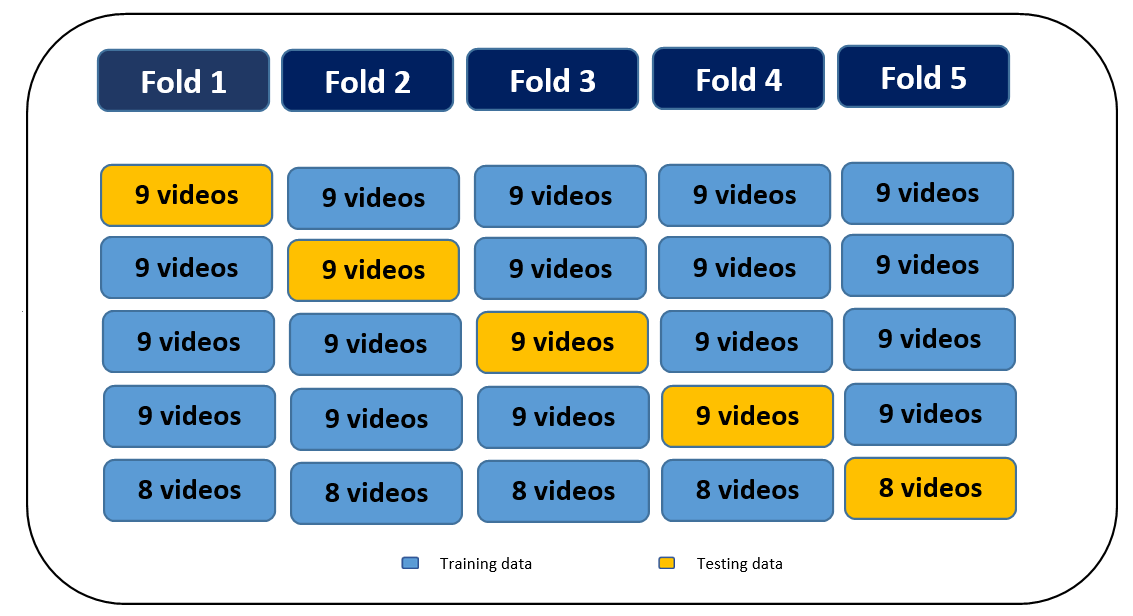
\includegraphics[width=1\textwidth]{Chapter5/Figs/crossVal.png}
%	\caption{Cross validation test}
%	\label{fig:VidcrossVal}
%\end{figure}
%%%%%%%%%%%%%%%%%%%%%%%%%%%%%%%%%%%%%%%%%%%%%%%%%%%%%%%%%%%%%%%%%%


\begin{figure}\centering
	\begin{subfigure}[b]{\textwidth}
		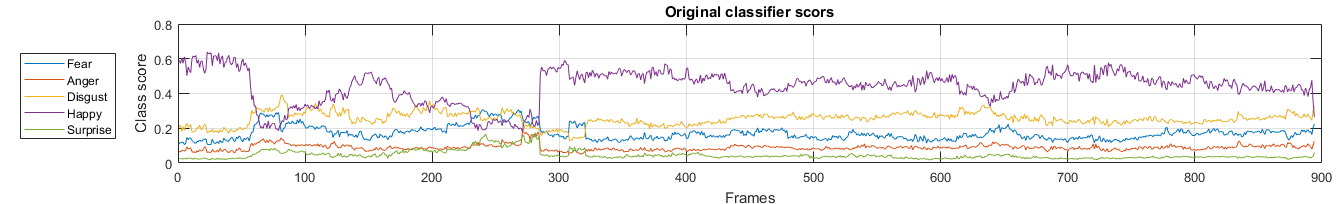
\includegraphics[width=1\textwidth]{Chapter5/Figs/DVD31_1_Pridect.png}
		
		\label{fig:database}
	\end{subfigure}\\[1em]
	%~ %add desired spacing between images, e. g. ~, \quad, \qquad etc. 
	%(or a blank line to force the subfigure onto a new line)
	\begin{subfigure}[b]{\textwidth}
		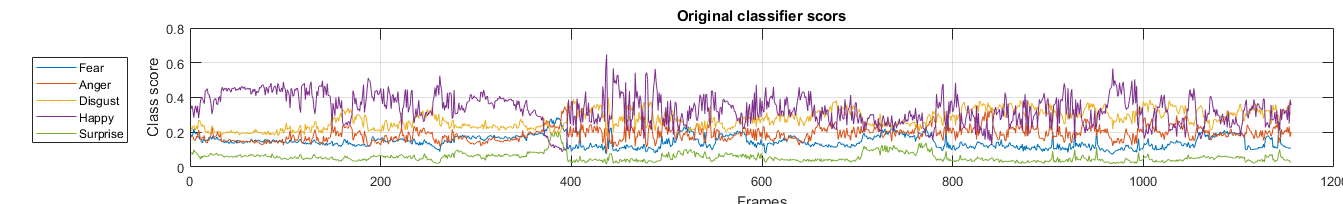
\includegraphics[width=1\textwidth]{Chapter5/Figs/DVD14_1_Pridect.png}
		
	\end{subfigure}
	\caption{Classifier prediction behaviour on two happy-labelled videos}\label{fig:Classifier_prediction}
\end{figure}

%
%%%%%%%%%%%%%%%%%%%%%%%%%%%%%%%%%%%%%%%%%%%%%%%%%%%%%%%%%%%%%%%%%%
% \begin{figure}[tb]
%\centering
%  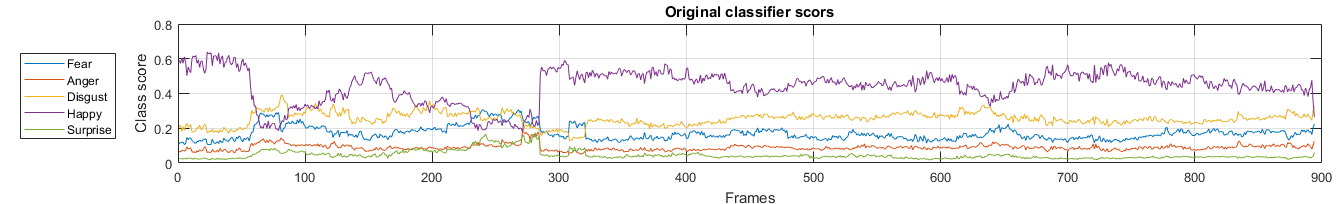
\includegraphics[width=1\textwidth]{Chapter5/Figs/DVD31_1_Pridect.png}
%  \caption{ Classifier prediction behaviour on happy-labelled video (DVD31\_1 contains 1056 frames).}
%         \label{fig:DVD31_1_Pridect}
%    \end{figure}
%%%%%%%%%%%%%%%%%%%%%%%%%%%%%%%%%%%%%%%%%%%%%%%%%%%%%%%%%%%%%%%%%%
%
%
%
%%%%%%%%%%%%%%%%%%%%%%%%%%%%%%%%%%%%%%%%%%%%%%%%%%%%%%%%%%%%%%%%%%
% \begin{figure}[tb]
%\centering
%  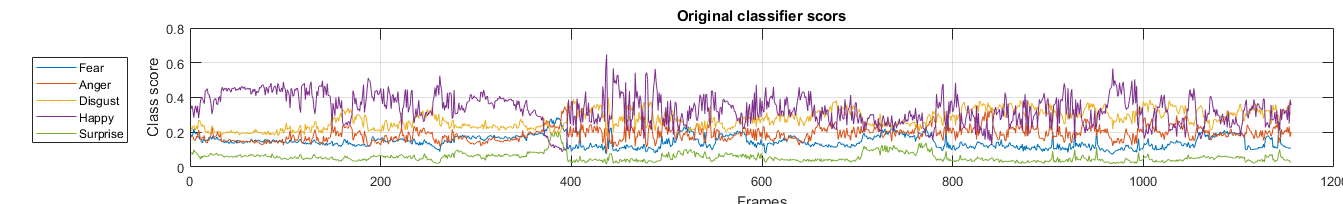
\includegraphics[width=1\textwidth]{Chapter5/Figs/DVD14_1_Pridect.png}
%  \caption{ Classifier prediction behaviour on happy-labelled video (DVD14\_1 contains 1056 frames).}
%         \label{fig:DVD14_1_Pridect}
%    \end{figure}







%\newpage
%%%%%%%%%%%%%%%%%%%%%%%%%Smoothing%%%%%%%%%%%%%%%%%%%%%%%%%%%%%%%%%%%%%%%%
%%%%%%%%%%%%%%%%%%%%%%%%%Smoothing%%%%%%%%%%%%%%%%%%%%%%%%%%%%%%%%%%%%%%%%

\section{Smoothing}
\label{smooting_PP}
It may be expected that the neighbouring frames in a video mostly contain the same facial expression. In other words, we assume that if the classifier has classified a frame as fear where the neighbouring frames were happy, it is likely to be a misclassification. To solve this problem, we suppose that smoothing the posterior probabilities of the classifier may reduce this misclassification and enhance the overall accuracy.

In smoothing, the individual data points (presumably because of misclassification) should be reduced, and the and points that are lower than the adjacent points are increased leading to a smoother data points\citep{simonoff2012smoothing}. 
Smoothing reduces the classifier's misclassification according to a span of classifiers score values. If the classifier classified a majority of 100 sequential frames as happy, and 7 (sequential or not) of this 100 classified as sad, it is most likely that there is an error in classifying those seven, so we can rely on the nearby frames to solve this misclassification.


 accuracy.%%%%%%%%%%%%%%%%%%%%%%%%%%%%%%%%%%%%%%%%%%%%%%%%%%%%%%%%%%%%%%%%%%
\begin{figure}[tb]
	\centering
	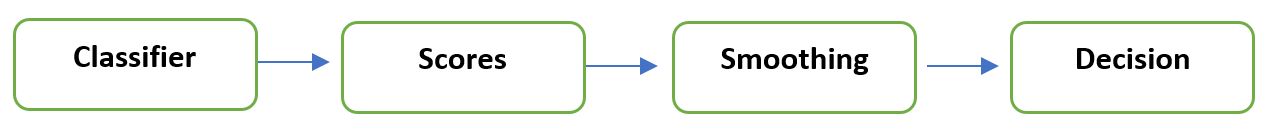
\includegraphics[width=1\textwidth]{Chapter5/Figs/SmoothPros.png}
	\caption{Decision making steps by smoothing the classifier scores ).}
	\label{fig:decisionsteps}
\end{figure}
%%%%%%%%%%%%%%%%%%%%%%%%%%%%%%%%%%%%%%%%%%%%%%%%%%%%%%%%%%%%%%%%%



\subsection{Smoothing techniques overview}
To smooth classifiers scores, several smoothing techniques have been tested: Locally weighted scatterplot smoothing (LOWESS and LOESS) and their robust versions,  the Savitzky-Golay filter \citep{savitzky1964smoothing},  and moving average smoothing.


\subsection*{Moving Average Filtering}
The moving Average Filtering smoothed value is determined by neighbouring data points
determined within a span. Moving Average Filtering smooth data by replacing each data point with the average of data points within the span. This method is described by equation \ref{eq:avarag_smoothing}.

%%%%%%%%%%%%%%%%%%%%%%%%%%%%%%%%%%%%%%%%%%%%%%%%%%%%%%%%%%%%%%%%%
\begin{equation}\label{eq:avarag_smoothing}
y_s (i) = \frac{1}{2N +1} (y(i + N)) + y(i + N -1) + ... + y(i + N - N)
\end{equation}
%%%%%%%%%%%%%%%%%%%%%%%%%%%%%%%%%%%%%%%%%%%%%%%%%%%%%%%%%%%%%%%%

where $y_s(i)$ is the smoothed value for the $i_th $data point, $N$ is the number of neighbouring data points on either side of $ys_(i)$, and $2N+1$ is the span.


\subsection*{Savitzky-Golay filter (SGF)}
The SGF is based on local least-squares polynomial approximation \citep{savitzky1964smoothing}. The smoothed signal g(t) is calculated by
convolving the signal f(t) with a smoothing (or convolution) function $h(t)$ for all observed data points $p$ where $f(m)$ is
the curve function at point m and $h(m - t) \neq  0 (3)$. The convolution function $h(t)$ is defined for each combination of
degree of the polynomial and window size \citep{press2007numerical}.




\subsection*{Local Regression Smoothing}
The names “lowess” and “loess” come from the term “locally weighted scatter plot smooth,” as the two methods use locally weighted linear regression to smooth data. The method starts with computing the regression weights for each data point in the data window (span). In the next step, a weighted linear least-squares regression is performed. For lowess, the regression uses the first-degree polynomial. For loess, the regression uses a second-degree polynomial. Finally, The smoothed value is given by the weighted regression at the predictor value of interest.
lowess and loess  methods have robust versions include an additional calculation of robust weights, which is resistant to outliers values in the span. 


%
%Figures \ref{fig:Moving_average}, \ref{fig:DVD14_1loess_smothing}, \ref{fig:DVD14_1lowess_smothing}, \ref{fig:DVD14_1sgolay_smothing}, \ref{fig:DVD14_1rlowess_smothing} and \ref{fig:DVD14_1rloss} show examples of classifiers votes smoothing for the video (DVD14\_ 1). Each figure shows the original data in the top, followed by smoothing results with two span values 0.3, and 0.9 respectively, at the bottom of the figure the original and smoothed classification accuracy.   

%\newpage
%
%\vfill




\subsection{Smoothing optimisation}

%

%\begin{figure}[ht]
%\centering
%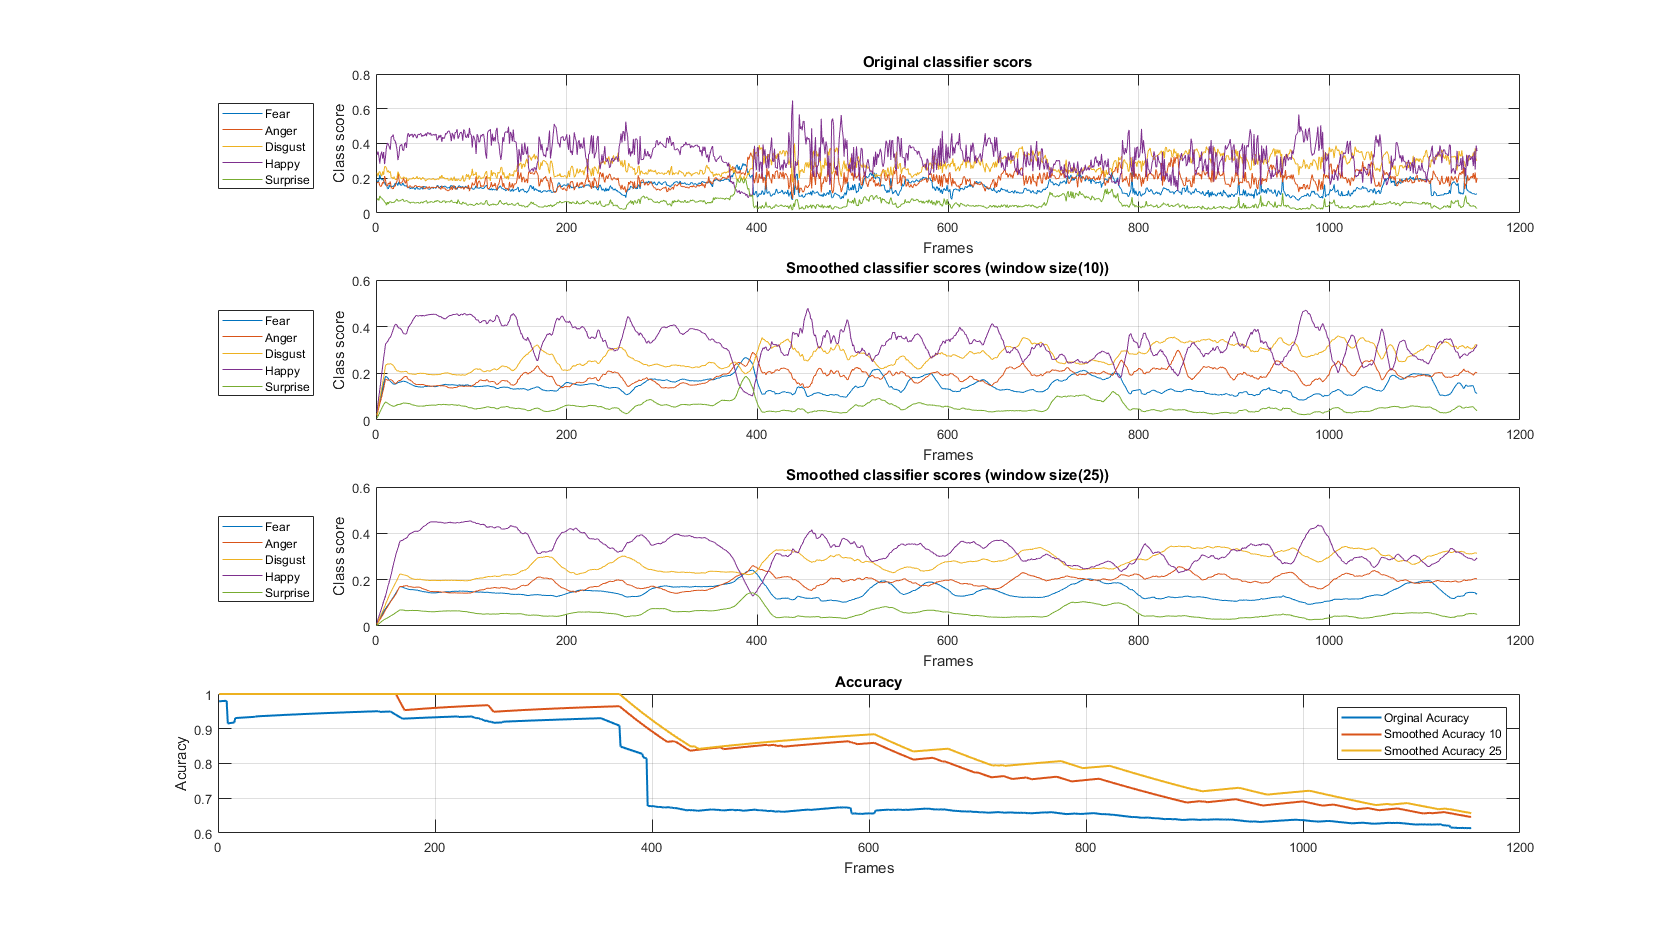
\includegraphics[width=.8\textwidth, center]{Chapter5/Figs/DVD14_1__1_1.png}
%\caption{\label{fig:TestOne}Moving average smoothing result for video DVD14\_1\_1.}
% \label{fig:Moving_average}
%
%\end{figure}
%
%\begin{figure}[h]
%\centering
%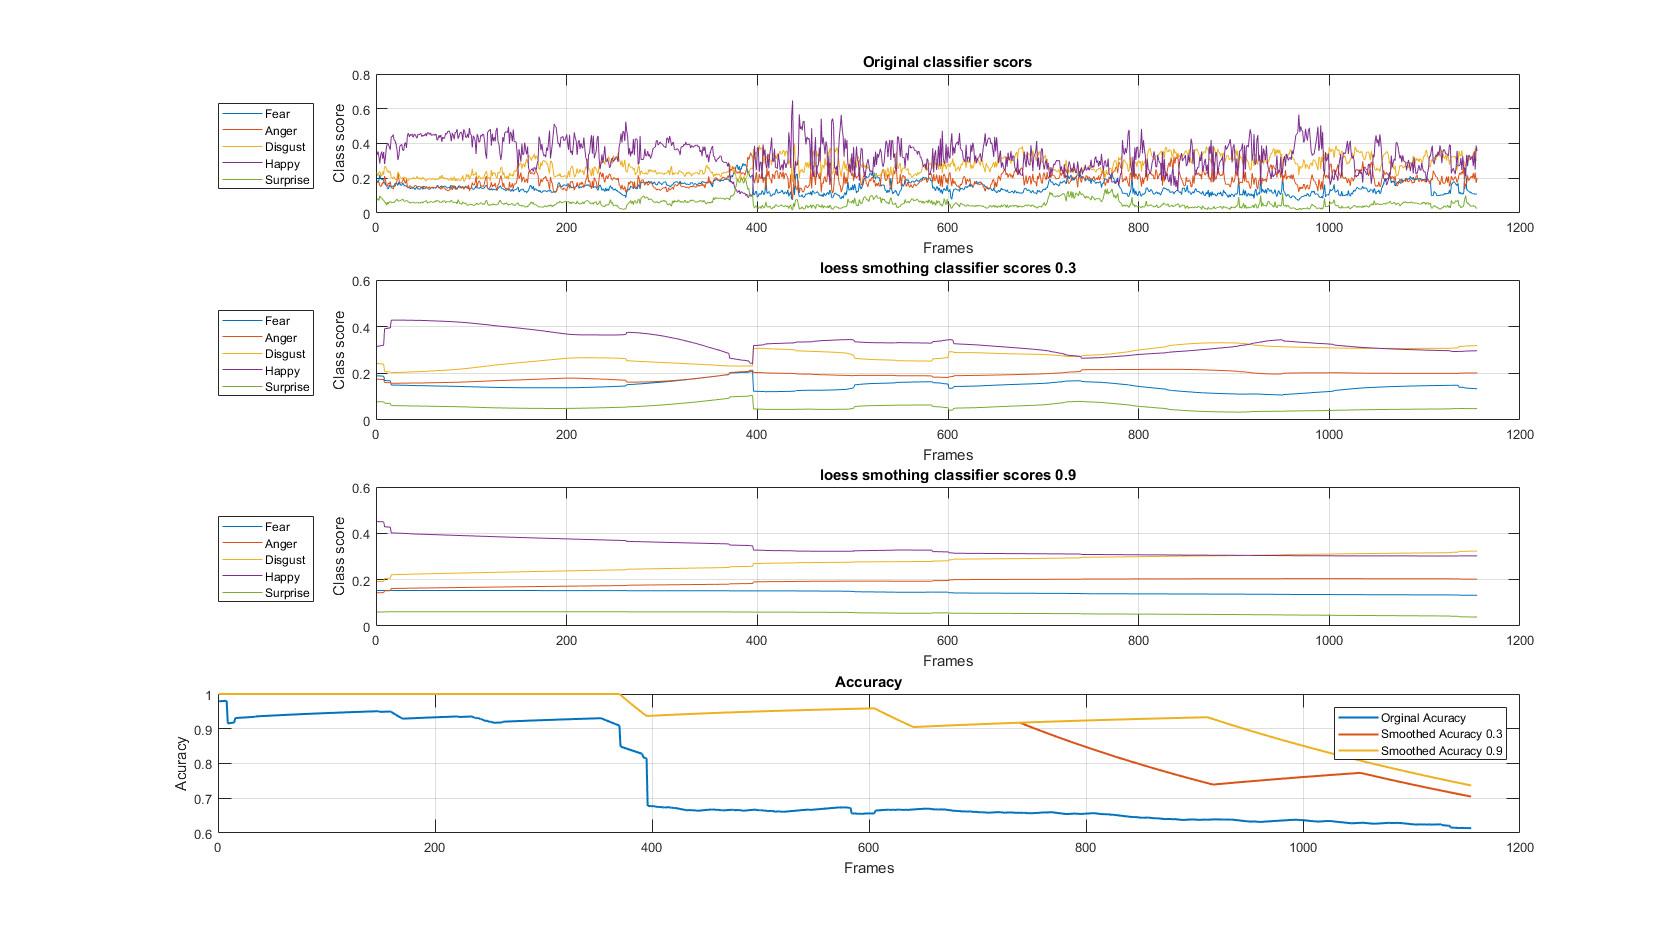
\includegraphics[width=.8\textwidth, center]{Chapter5/Figs/DVD14_1loess_smothing.png}
%\caption{\label{fig:TestOne}Loess (quadratic fit) smoothing result for video DVD14\_1\_1.}
% \label{fig:DVD14_1loess_smothing}
%\end{figure}

\begin{figure}[t]
	\centering
	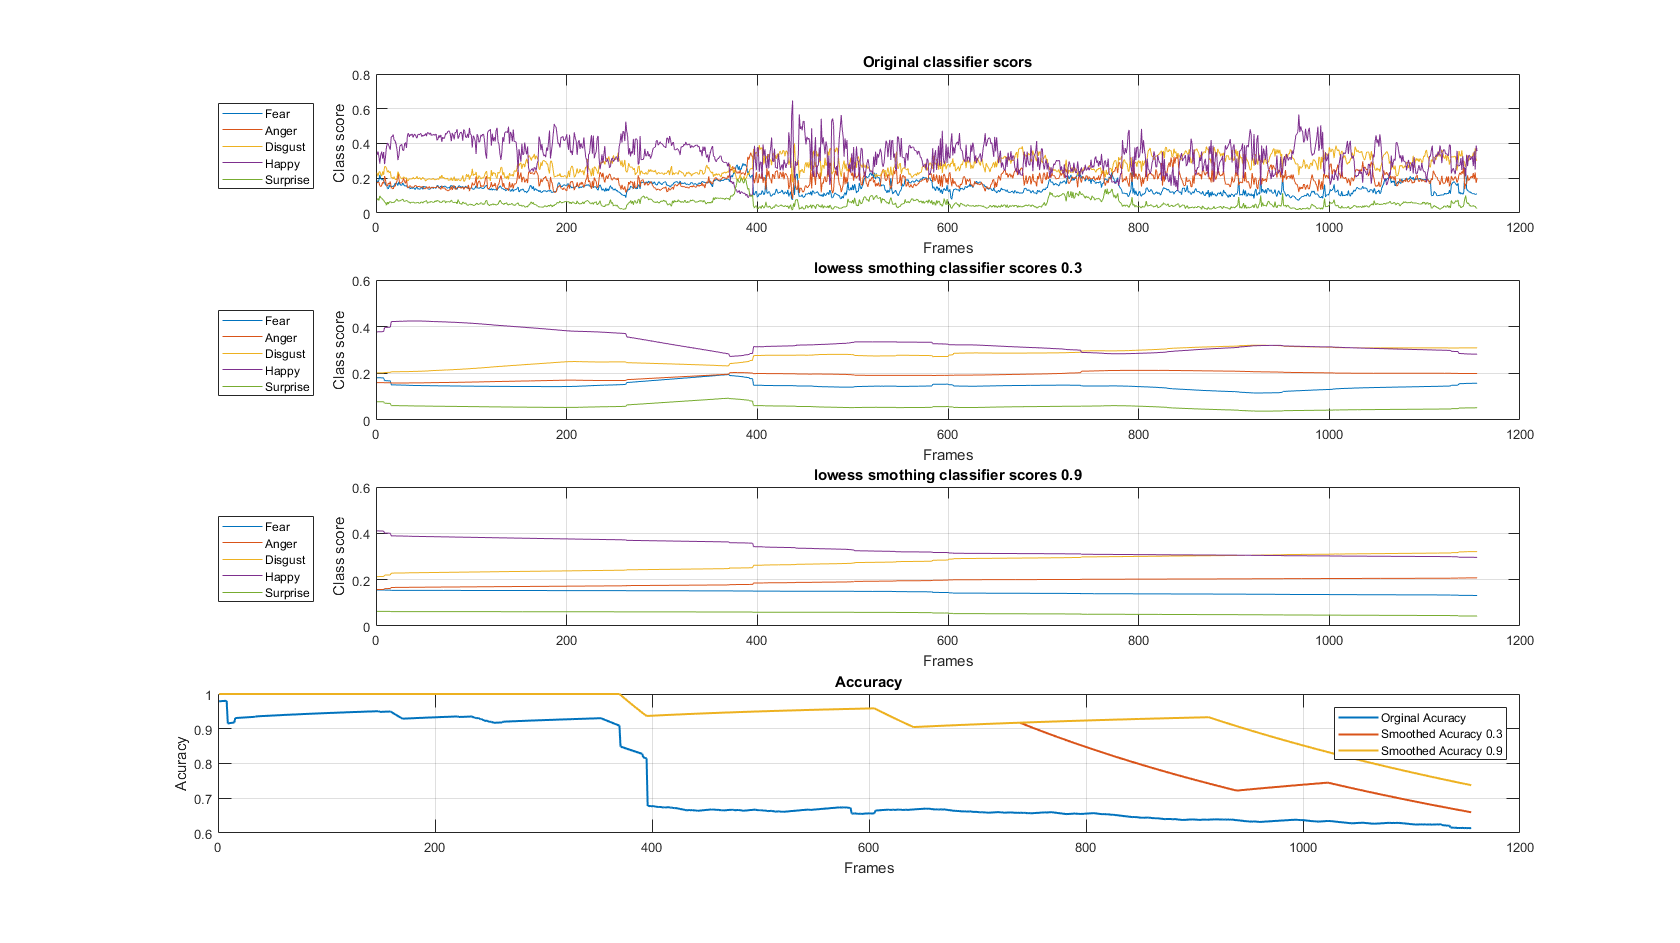
\includegraphics[width=1\textwidth, center]{Chapter5/Figs/DVD14_1lowess_smothing.png}
	\caption{\label{fig:TestOne}Lowess (linear fit) smoothing result for video DVD14\_1\_1.}
	\label{fig:DVD14_1lowess_smothing}
\end{figure}

%\begin{figure}[ht]
%\centering
%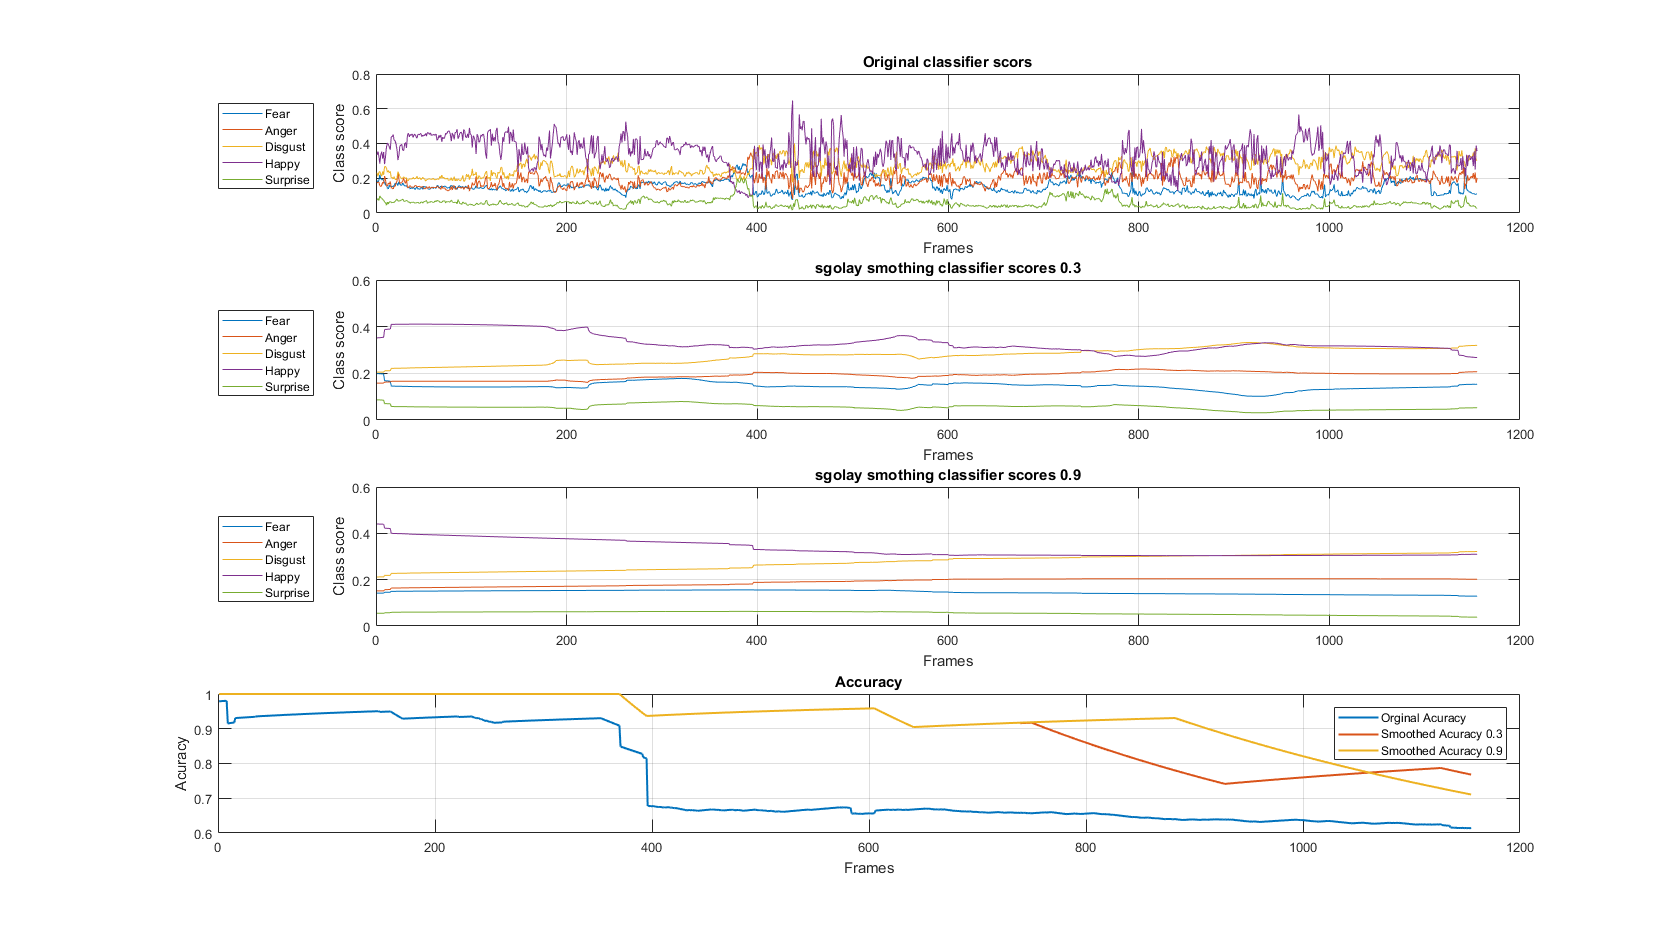
\includegraphics[width=.8\textwidth, center]{Chapter5/Figs/DVD14_1sgolay_smothing.png}
%\caption{\label{fig:TestOne}Savitzky-Golay smoothing result for video DVD14\_1\_1.}
%\label{fig:DVD14_1sgolay_smothing}
%\end{figure}
%
%
%\begin{figure}[ht]
%\centering
%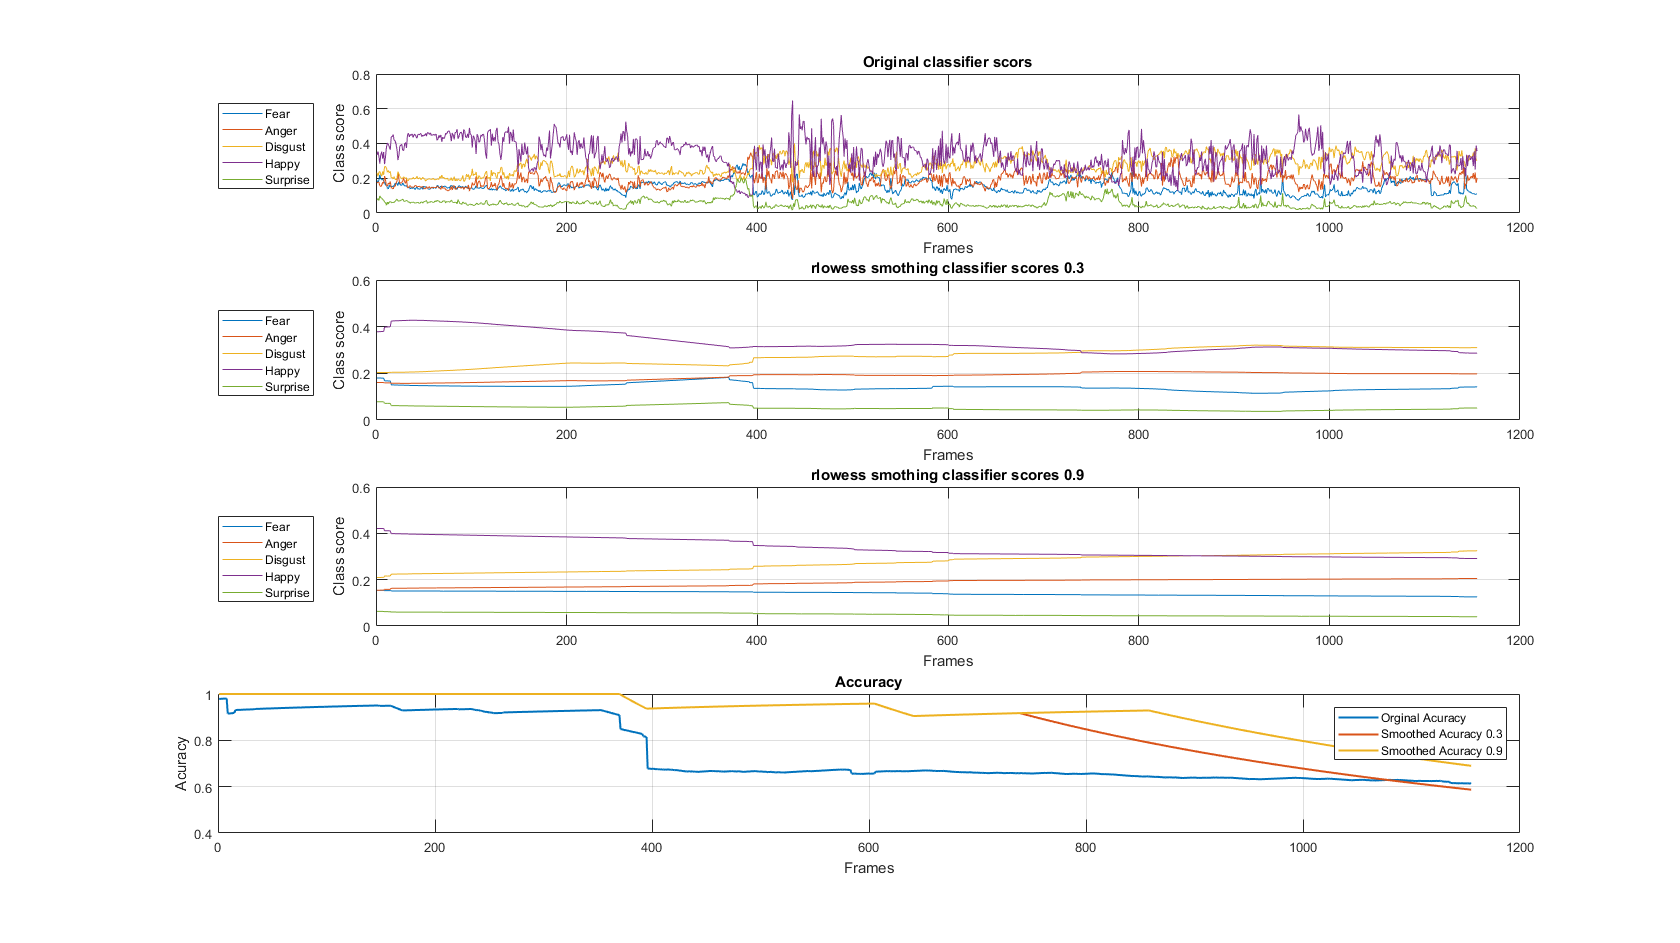
\includegraphics[width=.8\textwidth, center]{Chapter5/Figs/DVD14_1rlowess_smothing.png}
%\caption{\label{fig:TestOne}Robust Lowess (linear fit) smoothing result for video DVD14\_1\_1.}
%\label{fig:DVD14_1rlowess_smothing}
%\end{figure}
%
%
%
%\begin{figure}[ht]
%\centering
%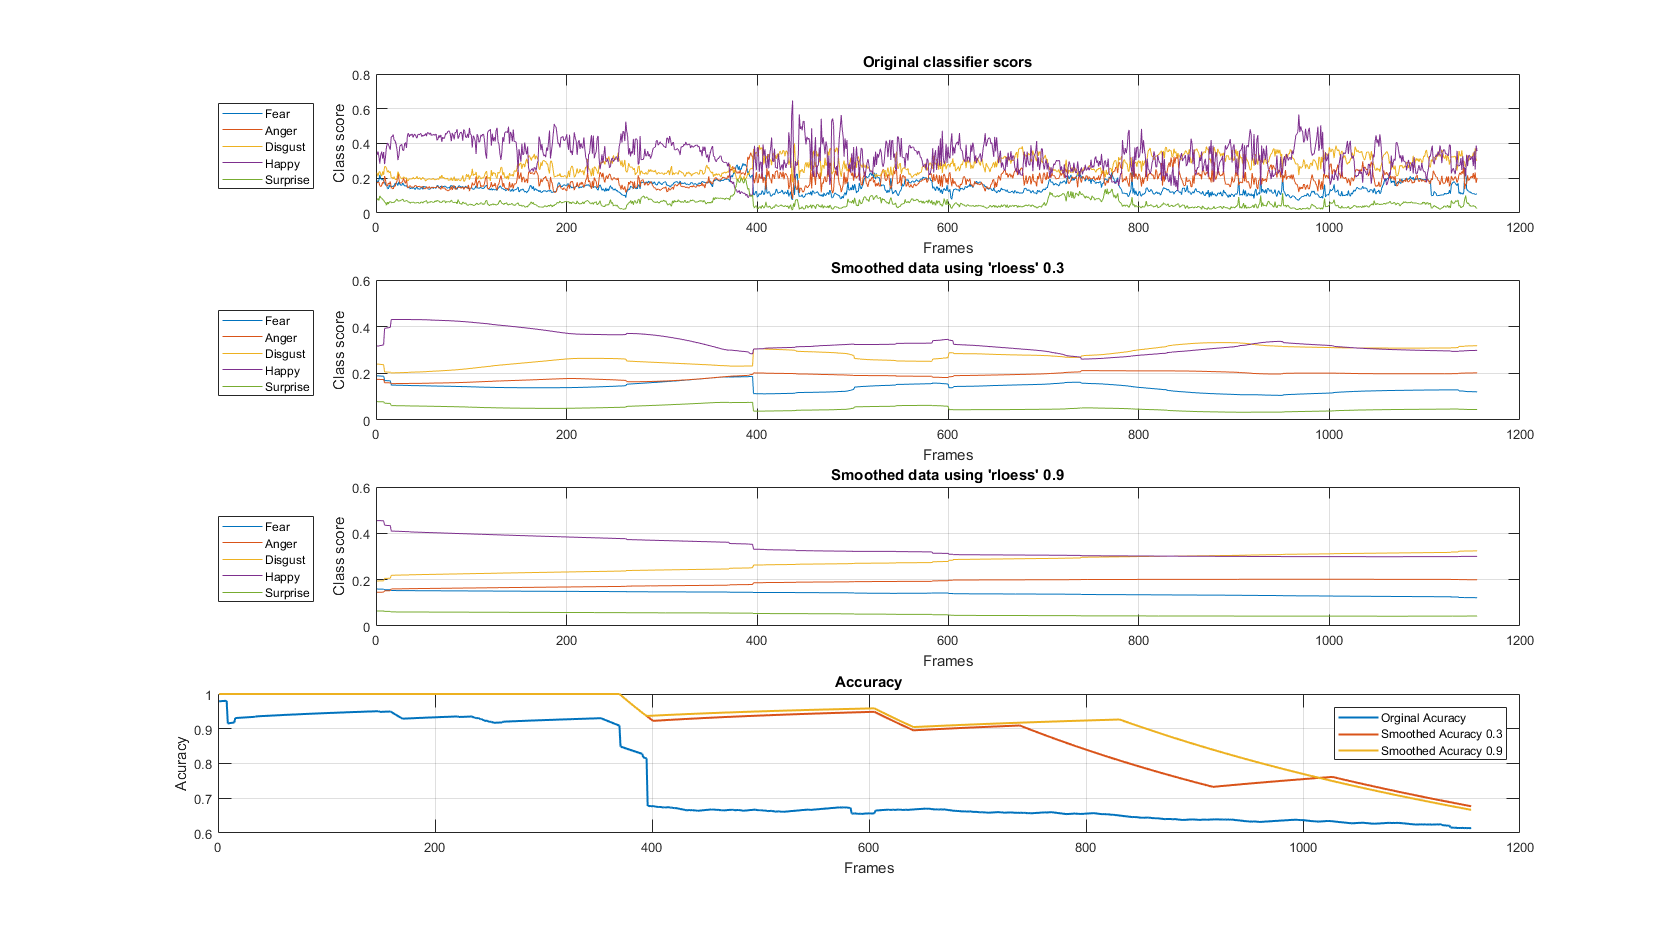
\includegraphics[width=.8\textwidth, center]{Chapter5/Figs/DVD14_1rloss.png}
%\caption{\label{fig:TestOne}Robust loess smoothing result for video DVD14\_1\_1.}
%\label{fig:DVD14_1rloss}
%\end{figure}


Figure \ref{fig:DVD14_1lowess_smothing} shows an example of mooting a short video called (DVD14\_ 1). The figure shows the original data in the top, followed by smoothing results with two arbitrary value span values. At the bottom of the figure, we can see the original and smoothed classification accuracy.


To smooth the classier scores, we need to find the optimal span value to get the best results. To achieve that, we use the Nelder–Mead method which is a popular numerical method to find the maximum or minimum of an objective function. However, the Nelder–Mead technique is a heuristic search method that can converge to non-stationary points on problems that can be solved by alternative methods \citep{barati2011parameter}.

By applying the Nelder–Mead on the classifier scores, we aim to find the optimal span which minimises the error. Table \ref{table:Optimising_of_smoothing} shows the optimisation results for the all the smoothing methods we mentioned. The table shows the best window size (span) gives the best accuracy for each smoothing method. We found that the Moving average and Lowess gives the best smoothing accuracy.  Moving average smoothing result was  87.9\% where Lowess was 87\%. 
\begin{figure}[t]
	\centering
	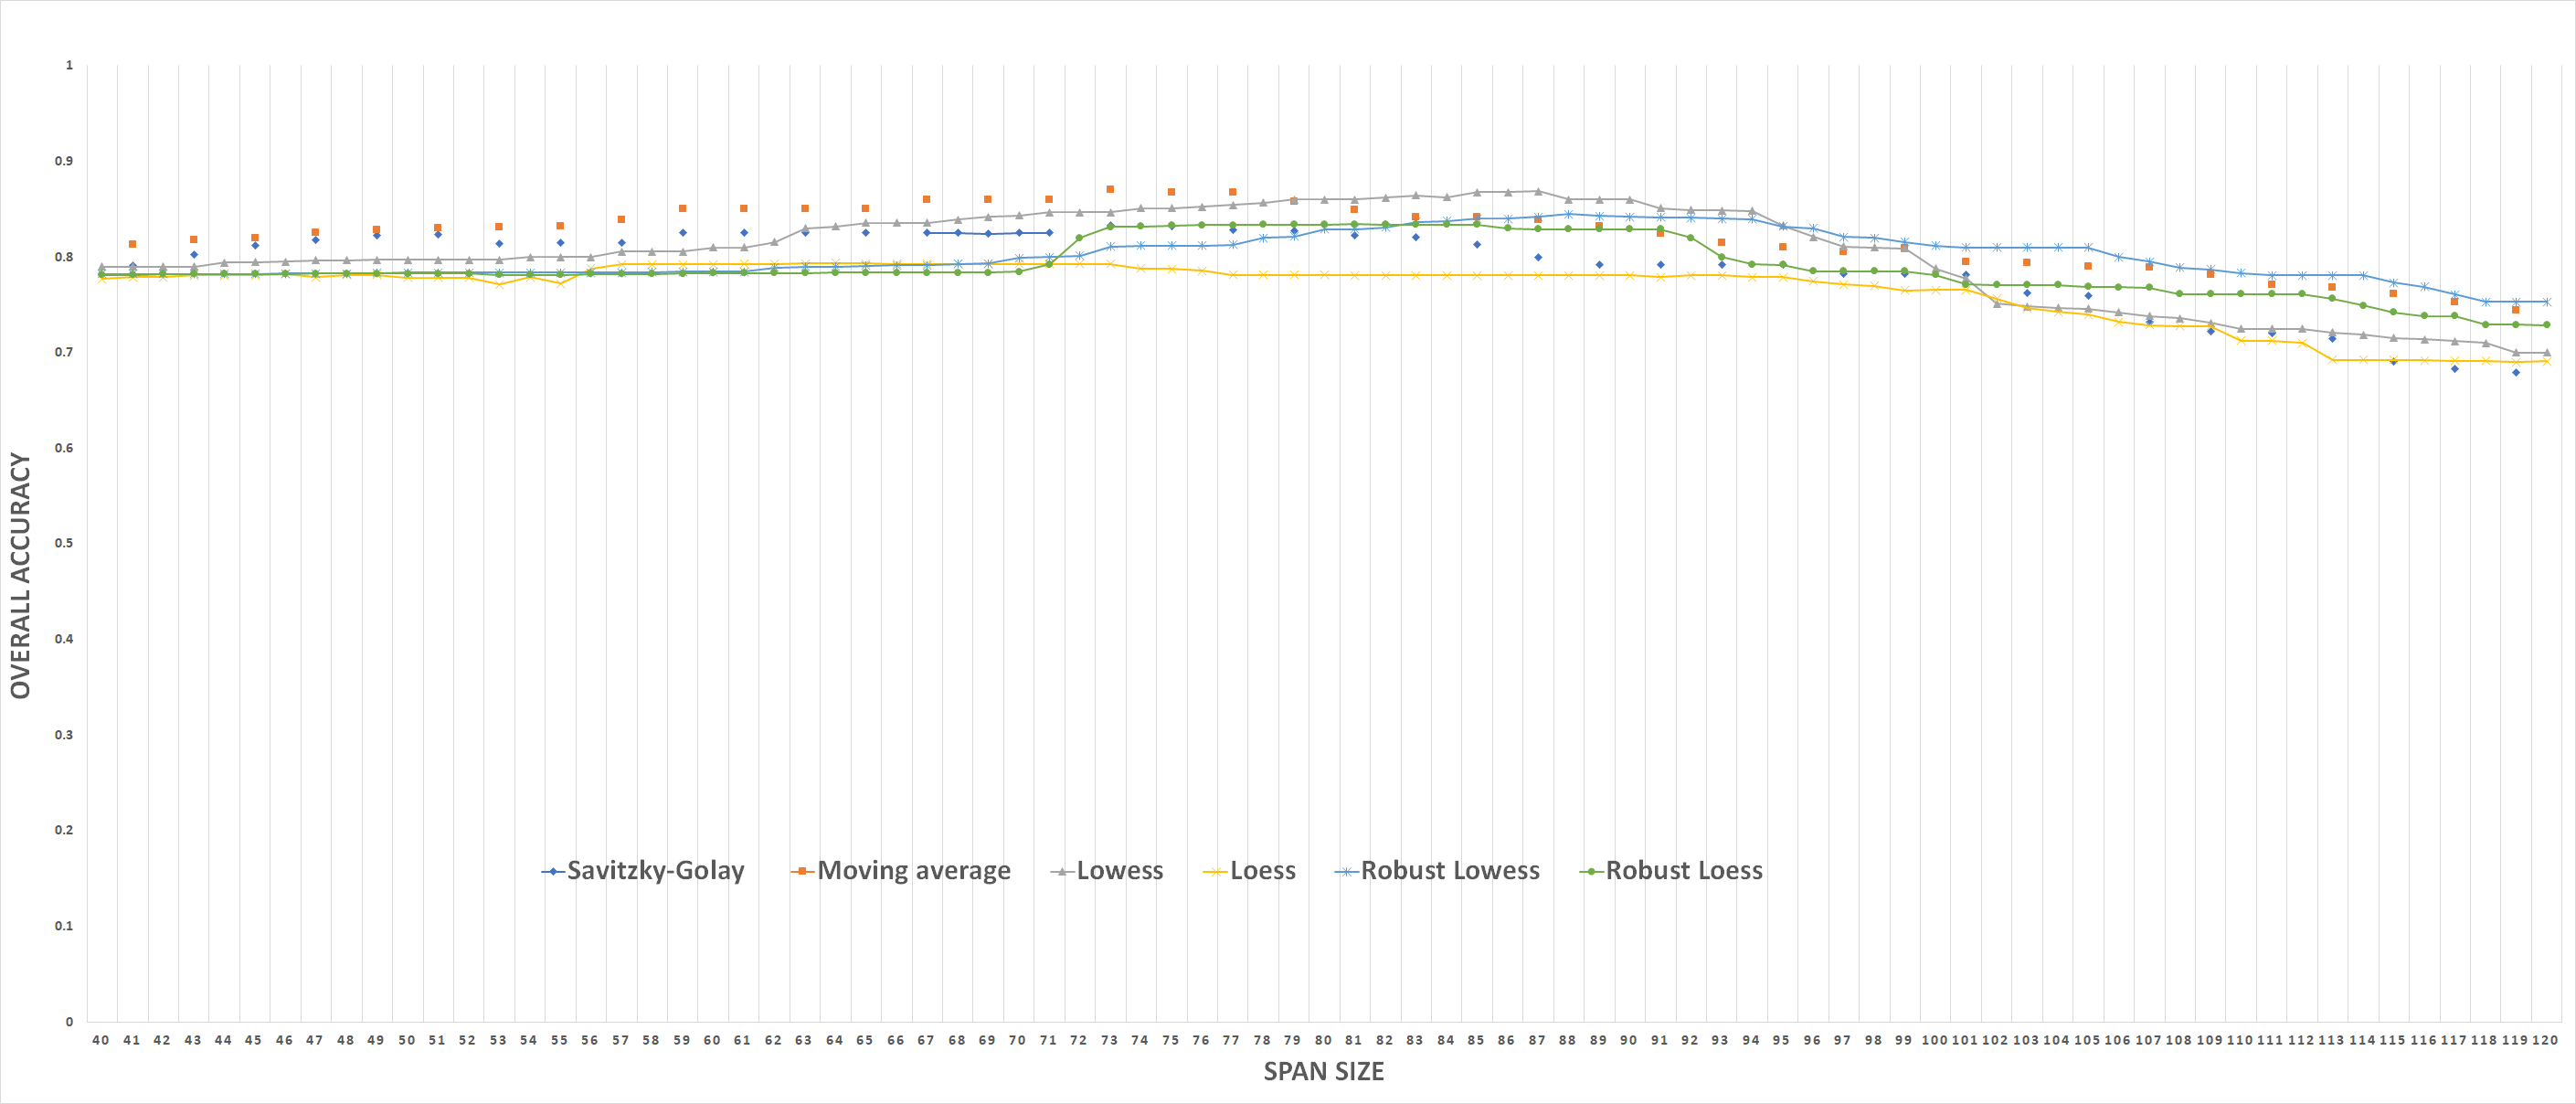
\includegraphics[width=1\textwidth, center]{Chapter5/Figs/SmoothOptimis.png}
	\caption{\label{fig:SmoothOptimis}The overall accuracy vs. smoothing span\_1\_1.}
	\label{fig:DVD14_1lowess_smothing}
\end{figure}
Figure \ref{fig:SmoothOptimis} illustrates the relationship between changing the smoothing span and the overall accuracy. We choosed a range between span size of 40 and 120 to show this figure, that means nearly 3 seconds and 8 seconds because the video rate is 15 frames per second.  All the optimal span sizes are in this size range. It is clear that all smoothing methods give the best accuracy before around span size 90, then they begin to go down.

Table \ref{tab:ConfusionmatrixAfterSmmoth} shows two confusion matrices for the same the DynEmo database and by applying 5-fold cross-validation after applying the smoothing method. The right confusion matrix show on RF classifier and the left shows 10-pairwise classifiers. 
We can see that something improved both methods with marked increase, from $79.6\%$ million (2015) to $87.1\%$  for the one classifier, which is an increase of nearly $8\%$, and from $83.4\%$  (2015) to $88.3\%$ for the one classifier which is an increase of nearly $5\%$.

All five facial expression rate have been rose be smoothing.  


%\begin{table}[H]
%\centering
%\caption{Optimising of smoothing span by Nelder–Mead (Staring point (0.5))}
%\label{table:Optimising_of_smoothing}
%\begin{tabular}{|l|c|c|}
%\hline
%\multicolumn{1}{|c|}{\textbf{Smoothing method}} & \textbf{Optimal smoothing span} & \textbf{Overall accuracy} \\ \hline
%Savitzky-Golay                                  & 0.538                            & 0.8329                    \\ \hline
%\textbf{Moving average}                         & \textbf{0.500}                   & \textbf{0.8709}           \\ \hline
%Lowess (linear fit)                             & 0.9750                           & 8688                      \\ \hline
%Loess (quadratic fit)                           & 0.500                            & 0.7935                    \\ \hline
%Robust Lowess (linear fit)                      & 0.9250                           & 0.8450                    \\ \hline
%Robust Loess (quadratic fit)                    & 0.7750                           & 0.8342                    \\ \hline
%Exponential filter                             & 0.5625                           & 0.7729                    \\ \hline
%\end{tabular}
%\end{table}


\begin{table}[t]
	\centering
	\caption{Optimising of smoothing span by Nelder–Mead (Staring point (0.5))}
	\label{table:Optimising_of_smoothing}
	\begin{tabular}{|l|c|c|}
		\hline
		\multicolumn{1}{|c|}{\textbf{Smoothing method}} & \textbf{Optimal smoothing (span)} & \textbf{Overall accuracy} \\ \hline
		Savitzky-Golay                                  & 69                            & 0.8329                    \\ \hline
		\textbf{Moving average}                         & \textbf{73}                   & \textbf{0.8709}           \\ \hline
		Lowess (linear fit)                             & 87                           & 0.8688                      \\ \hline
		Loess (quadratic fit)                           & 64                           & 0.7935                    \\ \hline
		Robust Lowess (linear fit)                      & 88                         & 0.8450                    \\ \hline
		Robust Loess (quadratic fit)                    & 81                        & 0.8342                    \\ \hline
	\end{tabular}
\end{table}


\begin{table}[H]
	\caption[caption]{Confusion matrix on the DynEmo database using proposed method after smoothing, the left is by one RF classifier, and the right 10-pairwise classifiers}
	\label{tab:ConfusionmatrixAfterSmmoth}
	\begin{minipage}{.5\linewidth}
		\centering
		Overall accuracy was $83.4\%$\\ (Normal RF classifier)\\[1mm]
		\resizebox{.95\textwidth}{!}{%
			\begin{tabular}{|c|c|c|c|c|c|}
				\hline
				& \textbf{FE}    & \textbf{AN}    & \textbf{DI}    & \textbf{HA}    & \textbf{SU}    \\ \hline
				\textbf{FE} & \textbf{0.457} & 0.045          & 0.198          & 0.099          & 0.201          \\ \hline
				\textbf{AN} & 0.043          & \textbf{0.766} & 0.145          & 0.012          & 0.034          \\ \hline
				\textbf{DI} & 0.085          & 0.117          & \textbf{0.679} & 0.000          & 0.119          \\ \hline
				\textbf{HA} & 0.014          & 0.009          & 0.018          & \textbf{0.938} & 0.021          \\ \hline
				\textbf{SU} & 0.083          & 0.009          & 0.071          & 0.022          & \textbf{0.815} \\ \hline
		\end{tabular}}
		
	\end{minipage}\hfill
	\begin{minipage}{.5\linewidth}
		\centering
		Overall accuracy was $88.3\%$ \\ (10-pairwise classifiers).\\[1mm]
		\resizebox{.95\textwidth}{!}{%
			\begin{tabular}{|c|c|c|c|c|c|}
				\hline
				& \textbf{FE}    & \textbf{AN}    & \textbf{DI}    & \textbf{HA}    & \textbf{SU}    \\ \hline
				\textbf{FE} & \textbf{0.543} & 0.058          & 0.157          & 0.054          & 0.188          \\ \hline
				\textbf{AN} & 0.031          & \textbf{0.826} & 0.124          & 0.010          & 0.010          \\ \hline
				\textbf{DI} & 0.064          & 0.174          & \textbf{0.641} & 0.000          & 0.121          \\ \hline
				\textbf{HA} & 0.013          & 0.011          & 0.009          & \textbf{0.952} & 0.016          \\ \hline
				\textbf{SU} & 0.115          & 0.026          & 0.065          & 0.010          & \textbf{0.784} \\ \hline
		\end{tabular}}
		
	\end{minipage} 
\end{table}

%
%\begin{table}[tb]
%\centering
%\textbf{
%\caption{Confusion matrix on DynEmo database using proposed method after finding the optimal smoothing span. Overall accuracy was $87.1\%$}\label{table:ConfusionmatrixAfterSmmith}}
%\begin{tabular}{|c|c|c|c|c|c|}
%\hline
%            & \textbf{FE}    & \textbf{AN}    & \textbf{DI}    & \textbf{HA}    & \textbf{SU}    \\ \hline
%\textbf{FE} & \textbf{0.457} & 0.045          & 0.198          & 0.099          & 0.201          \\ \hline
%\textbf{AN} & 0.043          & \textbf{0.766} & 0.145          & 0.012          & 0.034          \\ \hline
%\textbf{DI} & 0.085          & 0.117          & \textbf{0.679} & 0.000          & 0.119          \\ \hline
%\textbf{HA} & 0.014          & 0.009          & 0.018          & \textbf{0.938} & 0.021          \\ \hline
%\textbf{SU} & 0.083          & 0.009          & 0.071          & 0.022          & \textbf{0.815} \\ \hline
%\end{tabular}
%\end{table}
%

%\clearpage
\newpage

\section{Summary}
\label{sec:ch5_Summary}
In this chapter, we used an existing psychological facial emotion video dataset called the DynEmo to prepare it to be used for machine training and testing purposes. We prepared  44 videos to include 14543 frames distributed on five facial expressions as 8902 frames balled as happy, 313 fear, 2192 angry,  2665 surprise and  471 disgust. 
We use the method which was proposed in chapter \ref{Ch_4} to train random forests model with data from the DynEmo dataset mixed with some images from KDEF and eLFW. 
We tested some smoothing techniques to reduce the misclassification by smoothing the classifiers scores (posterior probability). To find the optimal smoothing span, we used the Nelder–Mead method to minimise the error.

As a result, like static images, our proposed system gives good results with videos. We found that applying smoothing methods with an optimal span value improved the performance of the classifiers by soothing their scores. As we have imposed, that the small misclassification should be fixed depending on the nearby frames.
The best span size is between 60 and 90, that means  4 to 6 seconds. This effects on the ability of our proposed system to work in real-time applications because it needs 4 to 6 seconds to give the results. The best smoothing method is moving average which needs nearly 5 seconds to give the best result.



%\begin{figure}[H]
%\centering
%\includegraphics[width=\textwidth]{Test1.jpg}
%\caption{\label{fig:TestOne}Testing result on video number one.}
%\end{figure}

%\iffalse
%%%%%%%%%%%%%%%%%%%%%%%%%%%%%%%%%%%%%%%%%%%%%%%%%%%%%%%%%%%%%%%%%%
%\begin{table}[H]
%\centering
%\textbf{
%\caption{Confusion matrices on LWF database using proposed method, trained with KDEF.}\label{LWFwithKDEF}}
%\fontsize{5pt}{5pt}
%\selectfont
%\begin{tabular}{@{}|l|c|c|c|c|c|@{}}
%\toprule
%            & \textbf{FE}    & \textbf{AN}    & \textbf{DI}    & \textbf{HA}     & \textbf{SU}    \tabularnewline \midrule
%\textbf{FE} & \textbf{0.491} & 0.019  & 0.062 & 0.034  & 0.391 \tabularnewline \midrule
%\textbf{AN} & 0.007 & \textbf{0.616} & 0.002 & 0.171  & 0.201 \tabularnewline \midrule
%\textbf{DI} & 0.084  & 0 & \textbf{0} & 0  & 0 \tabularnewline \midrule
%\textbf{HA} & 0 & 0 & 0 & \textbf{0}  & 0 \tabularnewline \midrule
%\textbf{SU} & 0 & 0 & 0 & 0 & \textbf{0} \tabularnewline \bottomrule
%\end{tabular}
%\end{table}
%%%%%%%%%%%%%%%%%%%%%%%%%%%%%%%%%%%%%%%%%%%%%%%%%%%%%%%%%%%%%%%%%%
%\fi

%\section{Weighted %pairwise classification}



